% Gerado por ferramentas/importar_relatorios.py a partir de CWRU/RELATORIO_CWRU-10.11.2026/RELATORIO_CWRU.tex.
% Revisado à mão na dissertação: edite este arquivo, não a fonte.
\subsection{Resultados}
\label{cwru:sec:resultados}

\subsubsection{Os \textit{hits} capturam a física do defeito, mas só com limiar flutuante}

A Figura~\ref{cwru:fig:sinais} mostra trechos de 60\,ms das quatro condições, com os \textit{hits} detectados. Na pista externa, os impactos são nítidos e espaçados de cerca de 9\,ms, mas o anel de cada impacto permanece acima de 0,3\,\(g\) por vários milissegundos. Na pista interna, com RMS de 0,58\,\(g\), o sinal fica acima do limiar fixo quase o tempo todo. Com limiar fixo, os impactos se fundem: na gravação IR de 0,007~polegada com carga 0, 95\,\% dos \textit{hits} foram truncados pela duração máxima, e em três das quatro gravações IR de 0,021~polegada, cerca de 50\,\%. É o mesmo regime de emissão contínua observado nos ensaios da bomba. Com o limiar flutuante, a fração truncada caiu para no máximo 1\,\% em todas as gravações.

\begin{figure}[htbp]
	\centering
	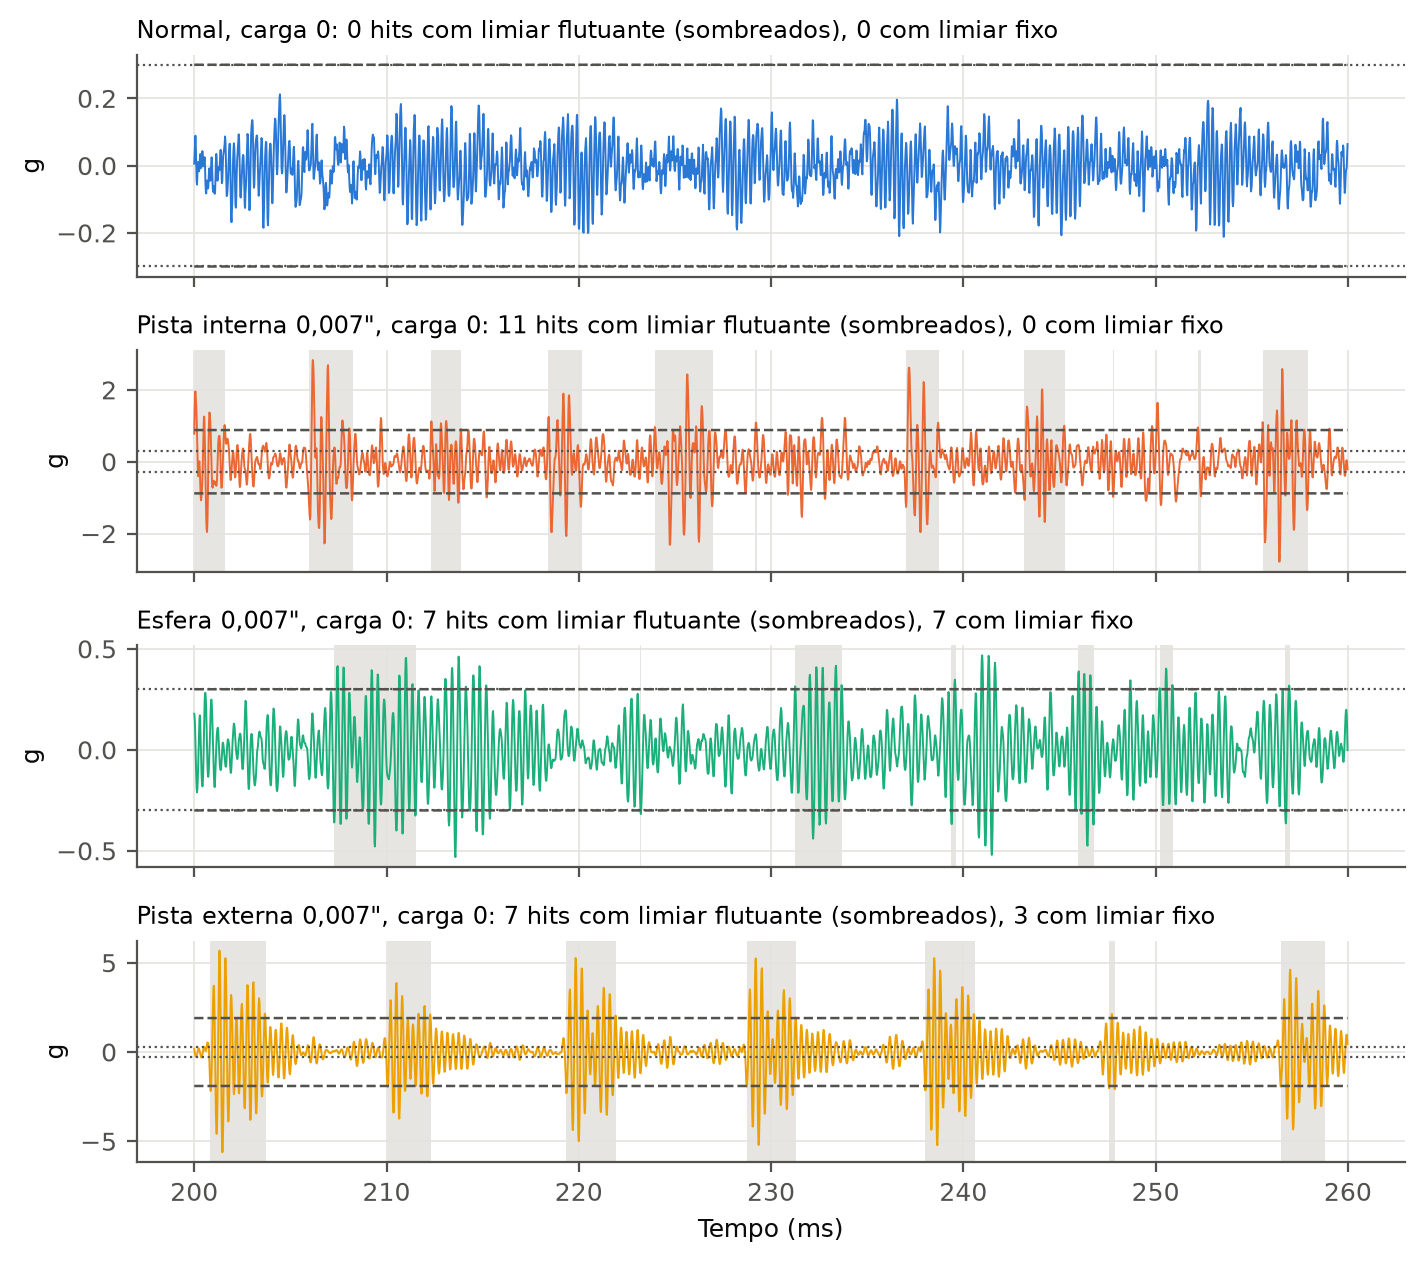
\includegraphics[width=\textwidth]{figs/cwru/fig_sinais_hits.png}
	\caption{Trechos de 60\,ms das quatro condições (carga 0, diâmetro de 0,007~polegada). Linhas pontilhadas: limiar fixo de 0,3\,\(g\); tracejadas: limiar flutuante. Áreas sombreadas: \textit{hits} detectados com o limiar flutuante.}
	\label{cwru:fig:sinais}
\end{figure}

A Figura~\ref{cwru:fig:ordem} mostra a ordem do intervalo entre \textit{hits}. Com limiar fixo, as distribuições são largas e têm picos espúrios perto de 1 e 2, que vêm de \textit{hits} fundidos e truncados. Com limiar flutuante, a pista externa concentra-se em 3,60 (BPFO = 3,58) e a pista interna em 5,27 (BPFI = 5,42); o pequeno desvio da pista interna é compatível com impactos perdidos quando o defeito sai da zona de carga. A esfera fica dispersa em torno de 5,5, longe de 2\(\times\)BSF = 4,71, o que concorda com a dificuldade conhecida de diagnosticar os defeitos de esfera dessa base \cite{smith2015}. Esse descritor é obtido sem FFT, apenas com os instantes dos \textit{hits}, o que reforça a importância do carimbo de tempo de \textit{hardware} ainda pendente no MOMEA.

\begin{figure}[htbp]
	\centering
	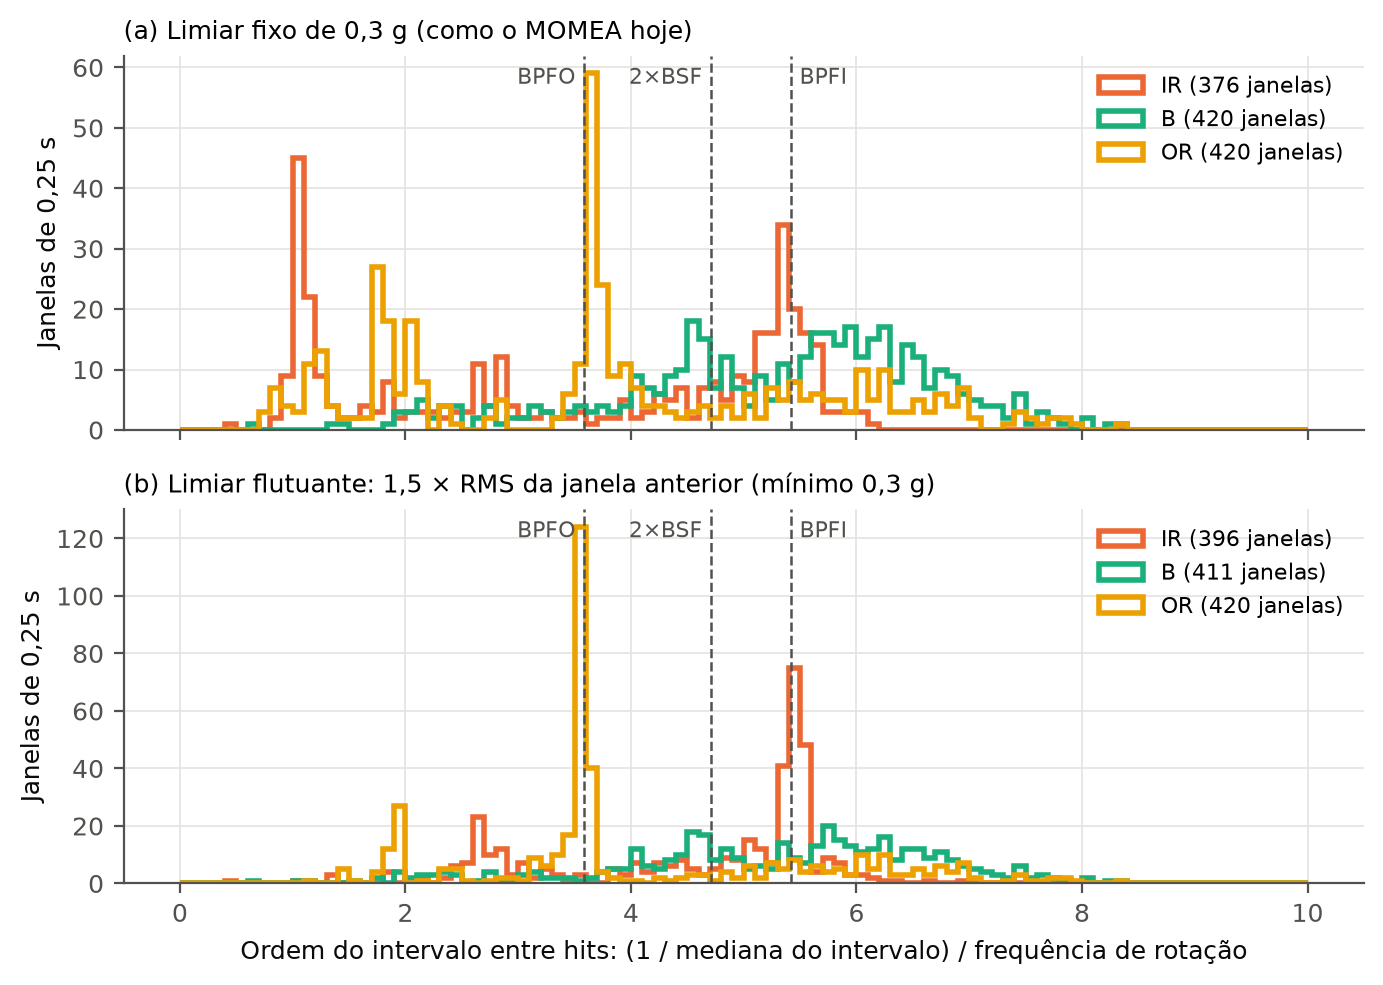
\includegraphics[width=\textwidth]{figs/cwru/fig_ordem_ihi.png}
	\caption{Ordem do intervalo entre \textit{hits} por janela, (a) com limiar fixo e (b) com limiar flutuante. Linhas tracejadas: frequências de defeito teóricas em múltiplos da rotação.}
	\label{cwru:fig:ordem}
\end{figure}

\subsubsection{A acurácia depende da validação}

A Figura~\ref{cwru:fig:acuracia} e a Tabela~\ref{cwru:tab:acuracia} resumem a classificação em quatro classes. Com janelas sorteadas, todos os grupos chegaram a 87--92\,\%, e as diferenças entre eles são pequenas. Deixar uma carga de fora quase não mudou o quadro (82--90\,\%), o que, à primeira vista, sugeriria boa generalização. Não é o caso: o teste ainda contém os mesmos rolamentos físicos, gravados em outra carga.

Quando o diâmetro inteiro sai do treino, a acurácia cai para perto do acaso nos descritores de amplitude: 21\,\% para os clássicos e 25\,\% para os \textit{hits} com limiar fixo, com a MLP. Os \textit{hits} com limiar flutuante sustentaram 46\,\% (53\,\% com RF), e o envelope, que mede diretamente as frequências de defeito, 63\,\%. Juntar todos os descritores não ajudou a MLP (41\,\%): os descritores de amplitude dominam o ajuste e não se transferem entre rolamentos, porque a severidade não é monotônica. Por exemplo, o defeito de 0,014~polegada na pista externa tem RMS de 4 a 8 vezes menor que os de 0,007 e 0,021. Na tarefa de dez classes, a queda das janelas sorteadas para a carga de fora foi um pouco maior (por exemplo, de 91 para 87\,\% com todos os descritores).

\begin{figure}[htbp]
	\centering
	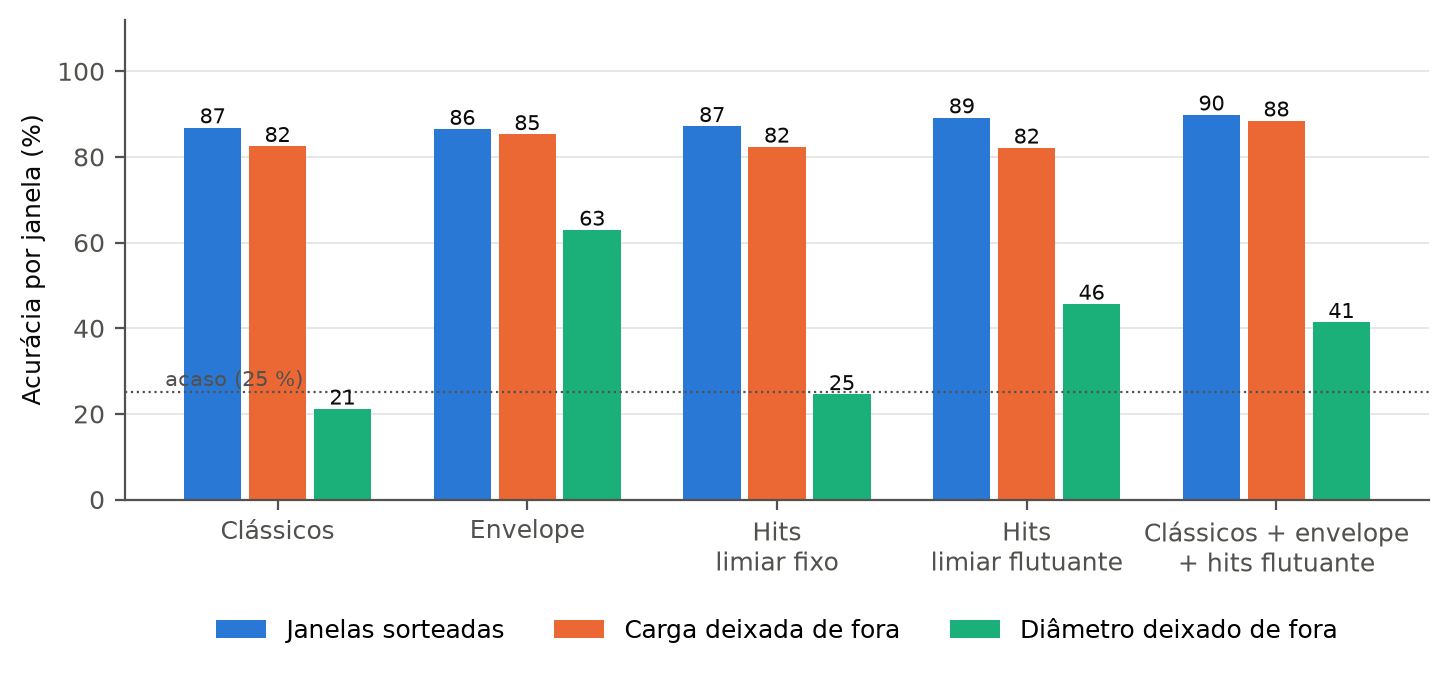
\includegraphics[width=\textwidth]{figs/cwru/fig_acuracia_validacoes.png}
	\caption{Acurácia por janela da MLP em quatro classes, por grupo de descritores e validação. A linha pontilhada marca o acaso (25\,\%).}
	\label{cwru:fig:acuracia}
\end{figure}

\begin{table}[htbp]
	\centering
	\small
	\caption{Acurácia por janela em quatro classes (entre parênteses, por gravação, com voto majoritário).}
	\label{cwru:tab:acuracia}
	\begin{tabular}{llccc}
		\toprule
		\textbf{Descritores} & \textbf{Modelo} & \textbf{Sorteada} & \textbf{Carga de fora} & \textbf{Diâmetro de fora} \\
		\midrule
		Clássicos & MLP & 86,8 (87,5) & 82,5 (82,5) & 21,2 (25,6) \\
		 & RF & 89,5 (92,5) & 86,4 (87,5) & 28,4 (28,2) \\
		Envelope & MLP & 86,5 (90,0) & 85,2 (90,0) & \textbf{62,9} (66,7) \\
		 & RF & 87,4 (90,0) & 85,8 (90,0) & 58,0 (59,0) \\
		\textit{Hits}, limiar fixo & MLP & 87,1 (90,0) & 82,3 (85,0) & 24,6 (20,5) \\
		 & RF & 88,7 (95,0) & 84,4 (80,0) & 35,3 (38,5) \\
		\textit{Hits}, limiar flutuante & MLP & 89,2 (92,5) & 82,1 (82,5) & 45,7 (43,6) \\
		 & RF & 90,5 (92,5) & 87,9 (90,0) & 53,3 (51,3) \\
		Todos (flutuante) & MLP & 89,8 (90,0) & 88,4 (87,5) & 41,4 (38,5) \\
		 & RF & 91,9 (90,0) & 89,6 (87,5) & 54,3 (51,3) \\
		\bottomrule
	\end{tabular}
\end{table}

A Figura~\ref{cwru:fig:confusao} mostra onde os erros se concentram, para os \textit{hits} com limiar flutuante. A máquina sã é sempre reconhecida, porque não gera \textit{hits}; o problema está em distinguir os defeitos entre si. Com o diâmetro de fora, a pista externa é confundida principalmente com a interna, e a esfera se divide entre as três classes de defeito.

\begin{figure}[htbp]
	\centering
	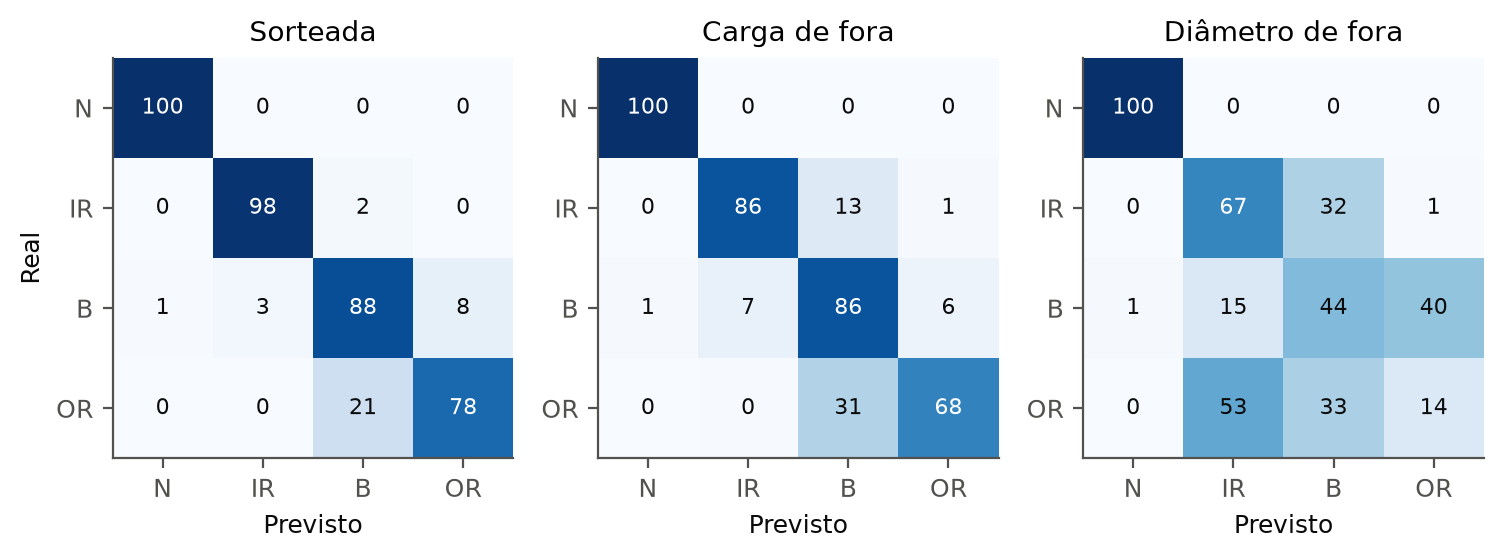
\includegraphics[width=\textwidth]{figs/cwru/fig_confusao_hits.png}
	\caption{Matrizes de confusão (\% por linha) da MLP com descritores de \textit{hits} e limiar flutuante, nas três validações.}
	\label{cwru:fig:confusao}
\end{figure}

\subsubsection{MLP int8}

Em cada parte da validação por carga, a MLP treinada foi quantizada para int8 com a mesma aritmética da implementação embarcada (Seção~\ref{sec:mm_embarcado}): escala de entrada fixa, pesos simétricos por camada e requantização inteira, com escalas calibradas apenas no treino da parte. A Tabela~\ref{cwru:tab:int8} mostra que a decisão int8 coincidiu com a de ponto flutuante em 98,4 a 100\,\% das janelas, e que a acurácia mudou no máximo 0,5 ponto percentual.

\begin{table}[htbp]
	\centering
	\small
	\caption{MLP em ponto flutuante e em int8 na validação por carga (quatro classes; faixas sobre as quatro partes).}
	\label{cwru:tab:int8}
	\setlength{\tabcolsep}{4pt}
	\begin{tabular}{lccccc}
		\toprule
		\textbf{Descritores} & \textbf{Entradas} & \textbf{MACs} & \textbf{Acc. float} & \textbf{Acc. int8} & \textbf{Concordância} \\
		\midrule
		\textit{Hits}, limiar flutuante & 14 & 3\,072 & 74,3--88,5\,\% & 73,8--88,2\,\% & 99,5--99,7\,\% \\
		Todos & 29 & 4\,032 & 86,5--90,5\,\% & 86,0--90,5\,\% & 98,4--100\,\% \\
		\bottomrule
	\end{tabular}
\end{table}

\subsubsection{Custo embarcado}

Os custos a seguir são estimativas derivadas dos ciclos medidos na simulação RTL da MicroBlaze a 100\,MHz (Seção~\ref{sec:mm_embarcado}), e não medições específicas para esta base:
\begin{itemize}
	\item \textbf{detecção dos \textit{hits}}: na lógica, como no MOMEA. A 48\,kHz, o detector é trivial para o FPGA;
	\item \textbf{descritores de \textit{hits}}: o custo medido foi de 4\,232 ciclos por \textit{hit} com FPU e 38\,287 sem. Na maior taxa observada (178 \textit{hits}/s), isso dá cerca de 0,8\,\% e 6,8\,\% da CPU, respectivamente;
	\item \textbf{MLP int8 com 14 entradas}: 3\,072 multiplicações-acumulações, ou cerca de 48 mil ciclos por janela (15,5 ciclos por operação, medidos), isto é, 0,5\,ms a cada 0,25\,s, ou 0,2\,\% da CPU;
	\item \textbf{envelope}: exige filtragem, transformada de Hilbert e FFT por janela. Com \(N = 16\,384\) pontos, cada FFT complexa custa cerca de \(5N\log_2 N \approx 1{,}1\) milhão de operações de ponto flutuante, e são necessárias pelo menos três. Isso dá da ordem de 3 a 4 milhões de operações por janela, ou 12 a 16 milhões por segundo. É inviável na MicroBlaze sem FPU e exigiria um núcleo de FFT na lógica.
\end{itemize}
Há, portanto, um compromisso claro: o envelope generaliza melhor entre rolamentos, mas custa uma FFT por janela; os \textit{hits} com limiar flutuante ficam a meio caminho, por uma fração do custo, e cabem na arquitetura atual do MOMEA.

% =======================================================================================================
\subsection{Discussão}
\label{cwru:sec:discussao}

\subsubsection{O que este estudo acrescenta à dissertação}

Os resultados reproduzem, numa base pública, as duas lições do estudo da bomba.
\begin{itemize}
	\item \textbf{A validação precisa separar as unidades físicas.} Janelas sorteadas e até cargas deixadas de fora deram 82--92\,\% com qualquer grupo de descritores, porque o modelo reconhece o rolamento, e não o tipo de defeito. Só separando os rolamentos a diferença entre os descritores aparece. É o mesmo padrão do LORO na bomba, em que a configuração das válvulas caiu de 89--95\,\% para 21--28\,\%. Na CWRU, porém, sabe-se que os defeitos são reais e localizados, de modo que a queda não pode ser atribuída à falta de efeito físico; ela vem da pouca diversidade de unidades (nove rolamentos com defeito e um são).
	\item \textbf{O limiar fixo do extrator falha diante de emissão contínua.} Com limiar fixo, os impactos se fundiram e foram truncados pela duração máxima, e os descritores de \textit{hits} ficaram no acaso fora da amostra. Com um limiar flutuante, os \textit{hits} recuperaram a periodicidade do defeito e a acurácia quase dobrou. Isso dá uma recomendação concreta para o MOMEA: oferecer um limiar flutuante na lógica, junto com a revisão do ganho já indicada pelos ensaios da bomba.
\end{itemize}

\subsubsection{Limitações}

\begin{itemize}
	\item Os sinais são de vibração, a 48\,kHz; nem os descritores nem as conclusões se transferem diretamente para EA de alta frequência ou para cavitação.
	\item O fator do limiar flutuante e o DDT foram escolhidos com base na concordância com as frequências de defeito, o que usa os rótulos; o ganho na validação por diâmetro pode estar ligeiramente otimista.
	\item Há apenas três partes na validação por diâmetro e nove rolamentos com defeito, de modo que as acurácias fora da amostra têm grande incerteza.
	\item Os defeitos são artificiais (eletroerosão) e únicos por condição; algumas gravações são atípicas, e os defeitos de esfera dessa base são sabidamente difíceis \cite{smith2015}.
	\item Os custos embarcados são estimativas a partir de medições em outra cadeia; o caminho completo para esta base não foi simulado em RTL.
\end{itemize}

% =======================================================================================================
